\section{Geometry of parameterised curves}
In the last section, we tried to describe the geometry of curves that can be described by implicit functions. There is another direction we can
generalise which will give us some similarly nice results.

A very simple example of the technique we want to study can be generted by recalling the definition of the functions $ \sin $ and $ \cos $. For
each angle $ t $ take the line $ \ell (t) $ through $ (0,0) $ which makes an anticlockwise angle $ t $ with the positive $ x$--axis, and call the
intersection point between $ \ell (t) $ and the unit circle $ P = (x,y) $; then set $ \sin t = y $ and $ \cos t = x $.

This definition sets up an exact correspondence between angles $ t $ ($ -\pi \leq t < \pi $) and points $ (x,y) $ on the unit circle ---
for each angle $ t $ we have precisely one point $ (\cos t, \sin t) $ on the circle, and for each point $ (x,y) $ on the circle
there is precisely one number $ t = \arcsin t = \arccos t $.

\begin{figure}
  \centering
  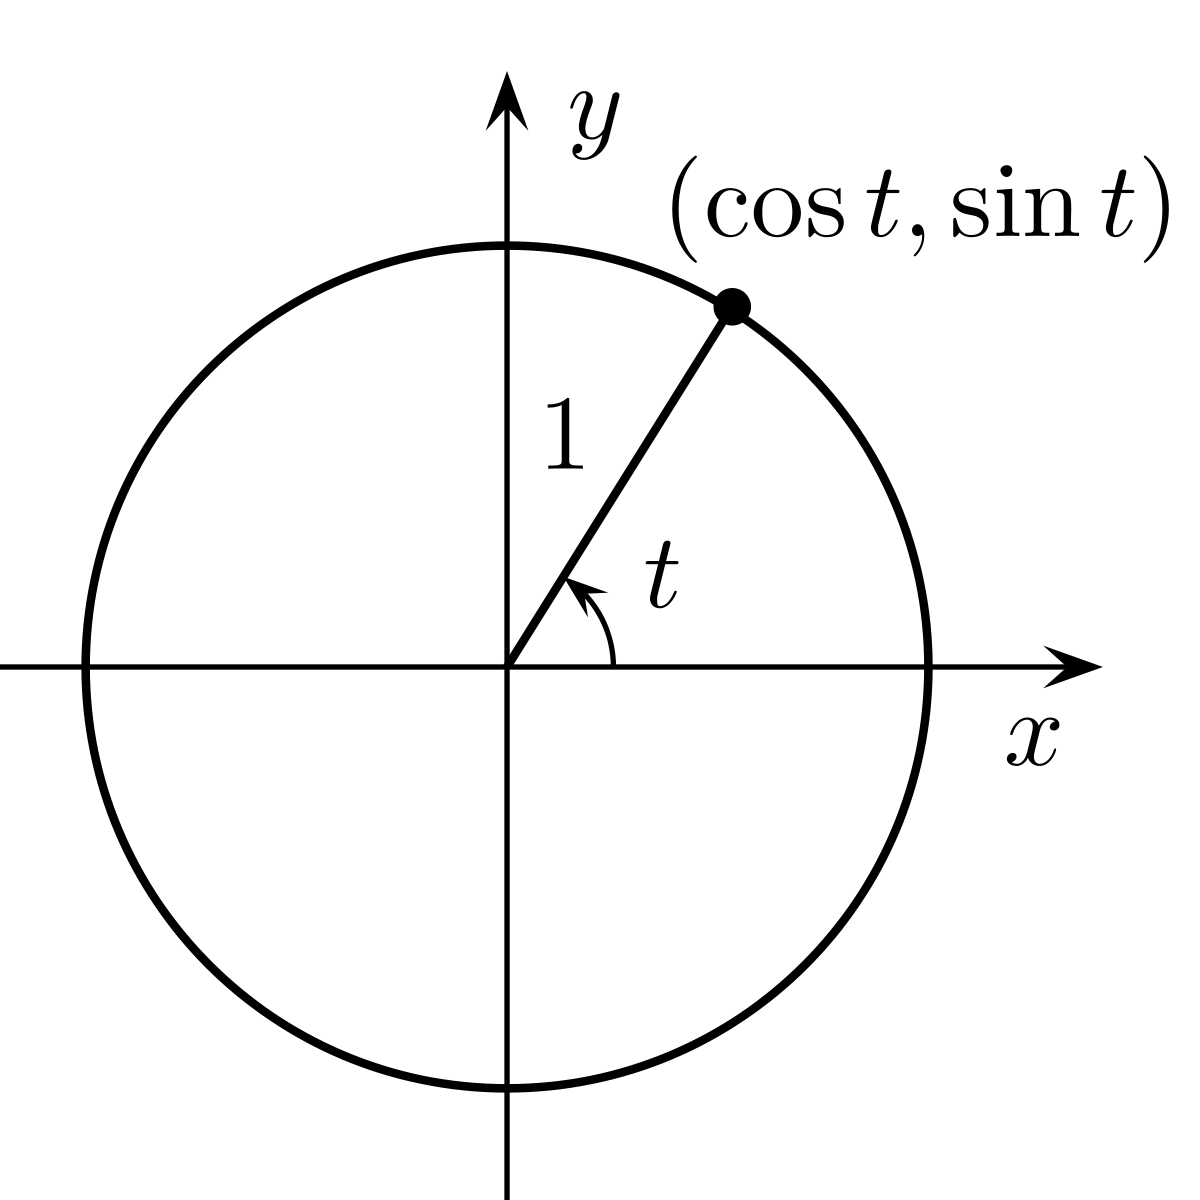
\includegraphics[width=0.2\textwidth]{circle}
  \caption{Parameterisation of the circle.\label{fig:param1}}
\end{figure}

In particular, we can say that the circle is the set of all points $ (x,y) = (\cos t, \sin t) $; and this is just a function (well, a pair
of functions) of one variable --- increasing $ t $ walks around the circle anticlockwise. We can differentiate to find that $ \od{x}{t} = -\sin t $
and $ \od{y}{t} = \cos t $; thus, by the chain rule,
\begin{equation}
  \od{y}{x} = \od{y}{t} \cdot \od{t}{x} = \frac{\cos t}{-\sin t} = -\frac{x}{y}.
\end{equation}

More generally, we want to study curves whose coordinates depend on a single parameter. If $ f $ and $ g $ are
differentiable functions, the curve $ \gamma $ given by
\begin{equation}
  \gamma(t) = (x,y) = (f(t), g(t))
\end{equation}
is called a \emph{parameterised curve}.

Recall that the \emph{implicit function theorem} states (roughly) that every curve can be sliced up into pieces which form the graphs of functions. For
each piece, $ y = g(f^{-1}(x)) $ and so
\begin{displaymath}
  \od{y}{x} = \frac{1}{f'(f^{-1}(x))} \cdot g'(f^{-1}(x)) = \frac{1}{f'(t)} \cdot g'(t) = \frac{1}{\od{x}{t}} \cdot \od{y}{t} = \od{y}{t} \cdot \od{t}{x}.
\end{displaymath}

In order to find the second derivative, we replace $ y $ with $ \od{y}{x} $:
\begin{displaymath}
  \dod[2]{y}{x} = \dod{\od{y}{x}}{x} = \left(\dod{}{t} \dod{y}{x}\right) \cdot \dod{t}{x}.
\end{displaymath}

\subsection{Exercises and Problems}
\begin{enumerate}
  \item In each case find $ \od{y}{x} $.
    \begin{enumerate}
      \item $ x = t\sin t $, $ y = t^2 + t $
      \item $ x = 2 \sec \theta $, $ y = 3\tan \theta $
      \item $ x = \cos \theta $, $ y = \cos 3\theta $
      \item $ x = e^{\sin \theta} $, $ y = e^{\cos \theta} $
    \end{enumerate}
  \item Find the equation of the chord joining the two points $ t = 2 $ and $ t = 4 $ on the
        curve $ (x,y) = (2t - 3, t^3 + 6) $.
  \item Determine the point(s) of intersection of the curves $ \gamma $ and $ \delta $ defined by
        \begin{align*}
          \gamma &: t \mapsto (t^2 - 2, t - 1),\\
          \delta &: t \mapsto (t, 2/t).
        \end{align*}
  \item
    \begin{enumerate}
      \item If $ y = 2t $ and $ x = 4t^2 $ define a curve, what is the gradient $ \od{y}{x} $ in terms of $ t $?
      \item Show that this curve is a parabola.
    \end{enumerate}
  \item A curve has parametric equations $ x = t^2 + 1 $ and $ y = t^3 + 2 $. Find $ \od{y}{x} $ and $ \od[2]{y}{x} $.
  \item Find the equation of the tangent to the curve $ t \mapsto (2x^2 + 1, t^3 - 1) $ at $ t = 2 $.
  \item If $ t \mapsto (x, y) $ is a parametric curve, find an expression for $ \od[3]{y}{x} $ analagous to that found for
        the second derivative.
  \item A curve, called a \textit{witch of Maria Agnesi}, consists of all possible positions of the point $ P $ in
        the diagram below. Graph the curve, show that the curve is given parametrically by $ (x, y) = (2a \cot \theta, 2a \sin^2 \theta) $, and
        find the derivative $ \od{y}{x} $.
        \begin{center}
          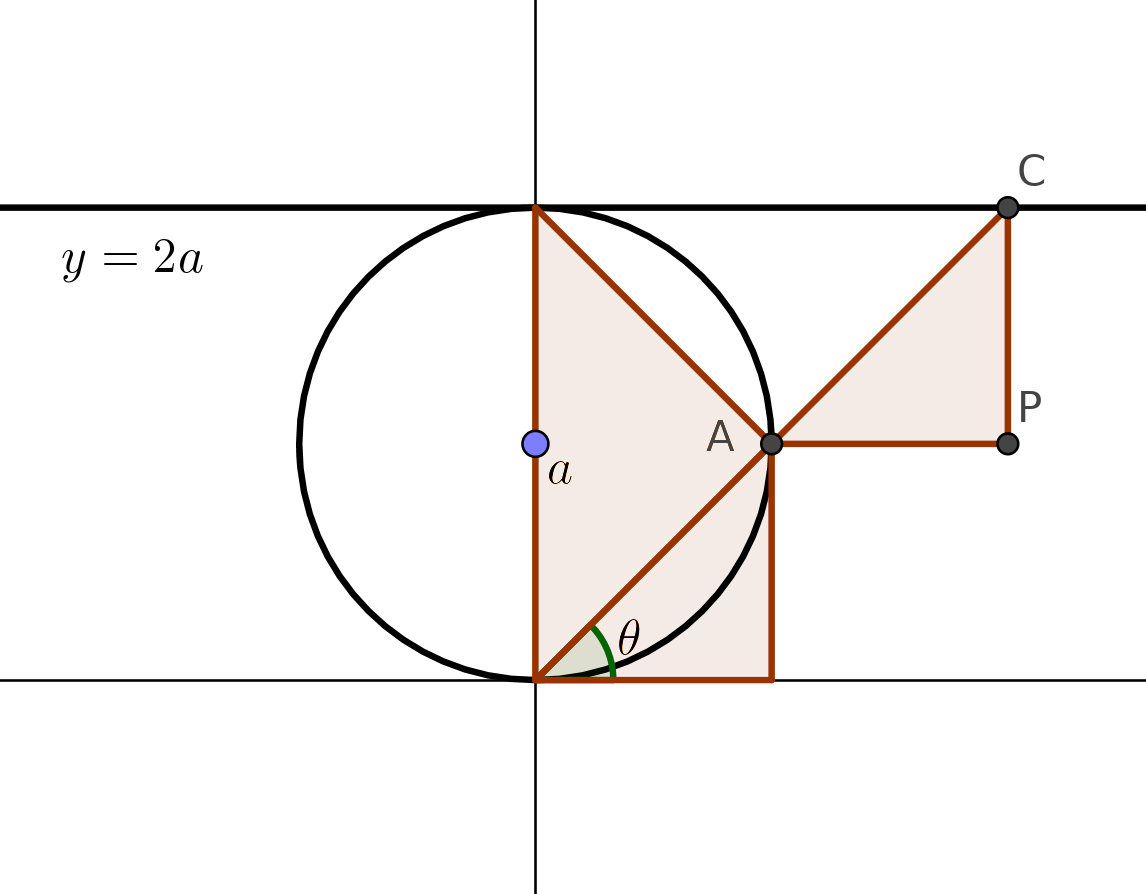
\includegraphics[width=0.5\textwidth]{agnesi-geom}
        \end{center}
  \item A particle moves through space over time; the position of the particle at time $ t $ is
        given by $ (3\sin t, 2\cos t) $ ($ 0 \leq t < 2\pi $).
    \begin{enumerate}
      \item What is the component of the acceleration of the particle in the $ x $ direction at $ t = \pi/4 $?
      \item At what times is the particle stationary in the $ x $ direction?
      \item Is the particle ever momentarily totally stationary?
    \end{enumerate}
  \item Find the rightmost point on the curve $ x = t - t^6 $, $ y = e^t $.
  \item For which values of $ t $ is the curve $ x = \cos 2t $, $ y = 3\cos t $ concave up?
  \item Show that the curve $ \gamma : t \mapsto (\cos t, \sin t \cos t) $ has two tangents at (0,0)
        and find their equations.
  \item
    \begin{enumerate}
      \item Give a second parameterisation of the unit circle $ x^2 + y^2 = 1 $ by considering the set of all lines through $ (-1,0) $.
      \item Give a parameterisation for the cubic $ x^3 - y^2 = 0 $. Find $ \od{y}{x} $ both using implicit differentiation and parametric
            differentiation, and check that the two results agree.
    \end{enumerate}
  \item Scholarship 2000: The piriform is the curve defined by the equation $ 16y^2 = x^3(8-x) $ where $ x \geq 0 $.
    \begin{enumerate}
      \item Show that
            \begin{displaymath}\begin{cases}
              x = 4(1 + \sin \theta)\\
              y = 4(1 + \sin \theta)\cos \theta.
            \end{cases}\end{displaymath}
            are parametric equations for the piriform.
      \item Find $ \od{y}{x} $ in terms of $ \theta $, and show that $ \theta = \frac{\pi}{6} $ is a stationary point of the curve.
    \end{enumerate}
  \item We define a surface $ C $ parametrically in terms of two parameters, $ t $ and $ \theta $:
        \begin{displaymath}
          (x,y,z) = (t, t \cos \theta, t \sin \theta).
        \end{displaymath}
    \begin{enumerate}
      \item Show that the Cartesian equation for this surface is $ x^2 = y^2 + z^2 $. (This is a cone.)
      \item Show that the intersection between $ C $ and the plane $ z = 2 $ is a hyperbola.
      \item For what angle $ \alpha $ does the intersection between $ C $ and the plane parametrically defined by
            \begin{displaymath}
              (x,y,z) = (u\tan \alpha + 1, u, v)
            \end{displaymath}
            (for parameters $ u $ and $ v $) become a parabola? (Hint: $ x = y \tan \alpha + 1 $, and $ z $ is arbitrary.)
    \end{enumerate}
\end{enumerate}

\subsection{References}

\subsection{Homework problems}
\begin{enumerate}
  \item F
\end{enumerate}
